% Dit werk is gelicenseerd onder de licentie Creative Commons Naamsvermelding-GelijkDelen 4.0 Internationaal. Ga naar http://creativecommons.org/licenses/by-sa/4.0/ om een kopie van de licentie te kunnen lezen.
\documentclass[t]{beamer}

% vaak gebruikte packages, nederlands
\usepackage[margin=2.5cm]{geometry}     % Marges instellen
\usepackage[dutch]{babel}               % Voor nederlandstalige hyphenatie (woordsplitsing)
\usepackage{amsmath,amsthm}             % Uitgebreide wiskundige mogelijkheden
\usepackage{url}                        % Om url's te verwerken
\usepackage{graphicx,subfigure}         % Om figuren te kunnen verwerken
\usepackage{color}
\usepackage{framed}
\usepackage{multicol}
\usepackage[small,bf,hang]{caption}     % Om de captions wat te verbeteren
\usepackage[utf8]{inputenc}             % Om niet ascii karakters rechtstreeks te kunnen typen
\usepackage{float}                      % Om nieuwe float environments aan te maken. Ook optie H!
\usepackage{flafter}                    % Opdat floats niet zouden voorsteken
\usepackage[section]{placeins}			% Om ervoor te zorgen dat floats binnen dezelfde section blijven
\usepackage[nottoc]{tocbibind}			% Bibliografie en inhoudsopgave in ToC; zie tocbibind.dvi
\usepackage{fancyhdr}                   % Voor fancy headers en footers
\usepackage{thmtools}                   % theorem tools
\usepackage{parskip}                    % Om paragrafen met een verticale spatie ipv horizontaal te laten beginnen
\usepackage[plainpages=false]{hyperref} % Om hyperlinks te hebben in het pdfdocument.



%%%%%%%%%%%%%%%%%%%%%%%%%%%%%%
% Algemene instellingen van het document.
%%%%%%%%%%%%%%%%%%%%%%%%%%%%%%
\renewcommand{\baselinestretch}{1.2} 	% De interlinie afstand wat vergroten.
\setcounter{MaxMatrixCols}{50}          % Max 20 kolommen in een matrix


%%%%%%%%%%%%%%%%%%%%%%%%%%%%%%
% Headers en footers
%%%%%%%%%%%%%%%%%%%%%%%%%%%%%%
\pagestyle{fancy}
\fancyhf{}
\renewcommand{\headrulewidth}{0pt}
\fancyhead[RO] {\rightmark}
\fancyhead[LE] {\leftmark}
\fancyfoot[RO,LE] {\thepage}

% no dot after chapter number
\renewcommand{\chaptermark}[1]{
	\markboth{\MakeUppercase{ \chaptername\ \thechapter\quad #1}}{}
}
% no dot after section number
\renewcommand{\sectionmark}[1]{
	\markright{\MakeUppercase{ \thesection\quad #1}}{}
}

% page header and footer style in mainmatter aanpassen
\let\newmainmatter\mainmatter
\renewcommand{\mainmatter}{

	\pagestyle{fancy}
	\fancyhf{}
	\renewcommand{\headrulewidth}{0pt}
	\fancyhead[RO] {\rightmark}
	\fancyhead[LE] {\leftmark}
	\fancyfoot[RO,LE] {\thepage}
	\fancyfoot[C]{\tiny{Brecht Baeten}}

	\newmainmatter
}
\let\newappendix\appendix
\renewcommand{\appendix}{
	\fancyfoot{}
	\fancyfoot[RO,LE] {\thepage}
	\newappendix
}


%%%%%%%%%%%%%%%%%%%%%%%%%%%%%%
% Nieuwe omgevingen
%%%%%%%%%%%%%%%%%%%%%%%%%%%%%%
\definecolor{shadecolor}{gray}{0.95}
\newcounter{voorbeeldcounter}[chapter]
\renewcommand{\thevoorbeeldcounter}{\thechapter.\arabic{voorbeeldcounter}}
\makeatletter
\newenvironment{voorbeeld}
{
\vspace{3mm}
\addtolength{\leftskip}{5mm}
\begin{shaded*}
\vspace{-3mm}
\refstepcounter{voorbeeldcounter}
\noindent
\textbf{Voorbeeld \thevoorbeeldcounter:\\}
%\vspace{-8mm}
%\begin{multicols}{2}
}
{
%\end{multicols}
\end{shaded*}
\addtolength{\leftskip}{-5mm}
}
\makeatother  
    
%%%%%%%%%%%%%%%%%%%%%%%%%%%%%%
% .svg commando's
%%%%%%%%%%%%%%%%%%%%%%%%%%%%%%
% nieuw commando om svg files dynamisch te updaten
%\newcommand{\executeiffilenewer}[3]{%
%\ifnum\pdfstrcmp{\pdffilemoddate{#1}}%
%{\pdffilemoddate{#2}}>0%
%{\immediate\write18{#3}}\fi%
%}
%% nieuw commando om. svg figuren in te voegen
%% Gebruik: \includesvg{path/filename.svg}
%\newcommand{\includesvg}[2][0]{%
%\executeiffilenewer{#2.svg}{#2.pdf}%
%{inkscape -z -C --file=#2.svg %
%--export-pdf=#2.pdf --export-latex}%
%\ifx#10
%	\let\svgwidth\undefined
%\else
%	\def\svgwidth{#1}
%\fi%
%\input{#2.pdf_tex}%
%\ifx \svgwidth\undefined
%\else
%	\let\svgwidth\undefined
%\fi%
%}

% nieuw commando om .fig figuren in te voegen
\newcommand{\includefig}[2][0]{%
\ifx#10
	\let\figwidth\undefined
\else
	\def\figwidth{#1}
\fi%
\input{#2.pdf_tex}%
\ifx \figwidth\undefined
\else
	\let\figwidth\undefined
\fi%
}

%%%%%%%%%%%%%%%%%%%%%%%%%%%%%%
% Packages
%%%%%%%%%%%%%%%%%%%%%%%%%%%%%%

%\usepackage{geometry}              	% 
\usepackage[dutch]{babel}               % Voor nederlandstalige hyphenatie (woordsplitsing)
\uselanguage{dutch}
\languagepath{dutch}
\usepackage{amsmath,amsthm}             % Uitgebreide wiskundige mogelijkheden
\usepackage{url}                        % Om url's te verwerken
\usepackage{graphicx,subfigure}         % Om figuren te kunnen verwerken
\usepackage[utf8]{inputenc}             % Om niet ascii karakters rechtstreeks te kunnen typen
\usepackage[section]{placeins}			% Om ervoor te zorgen dat floats binnen dezelfde section blijven
\usepackage{multicol}
\usepackage[absolute,overlay]{textpos}

%%%%%%%%%%%%%%%%%%%%%%%%%%%%%%
% Layout
%%%%%%%%%%%%%%%%%%%%%%%%%%%%%%
\usetheme{Frankfurt}
\usefonttheme[onlymath]{serif}
\AtBeginSection[]
{
  \begin{frame}
    \frametitle{Inhoud}
    \tableofcontents[currentsection]
  \end{frame}
}

\setbeamertemplate{navigation symbols}{}
\setbeamertemplate{footline}[page number]

%%%%%%%%%%%%%%%%%%%%%%%%%%%%%%
% Title
%%%%%%%%%%%%%%%%%%%%%%%%%%%%%%
\title{Fluïdummechanica}
\author{Brecht Baeten\inst{1}}
\institute{
	\inst{1}%
  		KU Leuven, Technologie campus Diepenbeek,\\ e-mail: brecht.baeten@kuleuven.be
}
\date{\today}
%%%%%%%%%%%%%%%%%%%%%%%%%%%%%%
% Omgevingen
%%%%%%%%%%%%%%%%%%%%%%%%%%%%%%


\subtitle{Hydrostatica}

\begin{document}
	\frame{\titlepage}
	\section{Inleiding}
		\begin{frame}
			\frametitle{Voorbeeld}
			\vspace{-0.5cm}
			\center
    		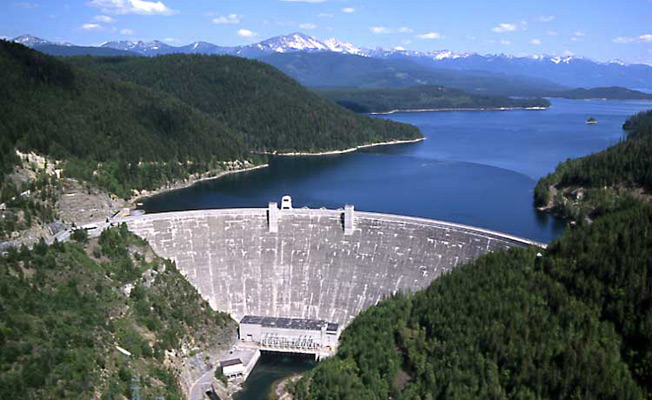
\includegraphics[height=0.8\textheight]{fig/hydrostatica/dam.jpg}\\
			\footnotesize{Bron: http://visitmt.com/}
			% Hungry horse dam, Montana
  		\end{frame}
%%%%%%%%%%%%%%%%%%%%%%%%%%%%%%%%%%%%%%%%%%%%%%%%%%%%%%%%%%%%%%%%%%%%%%%%%%%%%%%%%
  	\section{Hydrostatische druk}	
  		\begin{frame}
			\frametitle{Druk}
			\vspace{1cm}
			\center
			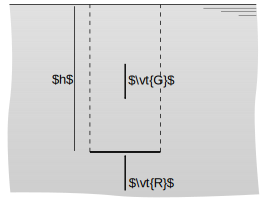
\includegraphics{fig/hydrostatica/oppervlak_in_stilstaande_vloeistof}
  		\end{frame}	
%%%%%%%%%%%%%%%%%%%%%%%%%%%%%%%%%%%%%%%%%%%%%%%%%%%%%%%%%%%%%%%%%%%%%%%%%%%%%%%%%
  	\section{Hydrostatische krachten}		
		\begin{frame}
			\frametitle{Krachten op rechte oppervlakken}
			\center
			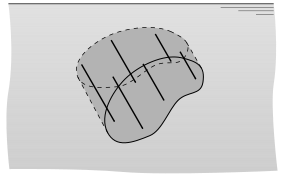
\includegraphics[scale=0.9]{fig/hydrostatica/grafische_weergave_integraal}
			\begin{itemize}
				\pause
				\item De resultante kracht is het volume van de figuur gevormd door de druk op het oppervlak uit te zetten
				\pause
				\item Het aangrijpingspunt is de projectie van het zwaartepunt van de figuur gevormd door de druk op het oppervlak uit te zetten
			\end{itemize}
  		\end{frame}
%%%%%%%%%%%%%%%%%%%%%%%%%%%%%%%%%%%%%%%%%%%%%%%%%%%%%%%%%%%%%%%%%%%%%%%%%%%%%%%%%
  		\begin{frame}
			\frametitle{Toepassing}
			\vspace{1cm}
			\center
			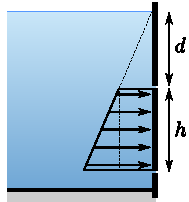
\includegraphics{fig/hydrostatica/kracht_op_luik}
			
			Bereken de resulterende kracht en het aangrijpingspunt
		\end{frame}
%%%%%%%%%%%%%%%%%%%%%%%%%%%%%%%%%%%%%%%%%%%%%%%%%%%%%%%%%%%%%%%%%%%%%%%%%%%%%%%%%	
  		\begin{frame}
			\frametitle{Krachten op gebogen oppervlakken oppervlakken}
			\center
			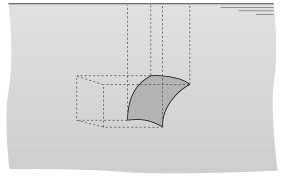
\includegraphics[scale=0.9]{fig/hydrostatica/kracht_gebogen_oppervlak_vereenvoudigd_3d}
			\pause
			\vspace{-0.5cm}
			\begin{equation}
				\diff F_r = -p \vt{n} \cdot \vt{r} \diff A
			\end{equation}
			\vspace{-0.7cm}
			\begin{itemize}
				\pause
				\item De horizontale kracht is gelijk aan de horizontale kracht op de projectie van het oppervlak op een verticaal vlak
				\pause
				\item De verticale kracht is gelijk aan het gewicht van het fluïdum dat zich boven het oppervlak kan bevinden
			\end{itemize}
  		\end{frame}
%%%%%%%%%%%%%%%%%%%%%%%%%%%%%%%%%%%%%%%%%%%%%%%%%%%%%%%%%%%%%%%%%%%%%%%%%%%%%%%%%
\end{document}